 \documentclass[dvipsnames,svgnames,beamer]{beamer}

\usetheme{Boadilla}
%\usecolortheme{seahorse}

\usepackage[utf8]{inputenc}

\usepackage{cancel}

\usepackage{lib}
\usepackage{tikz}
\usetikzlibrary{arrows.meta}
\tikzset{%
  >={Latex[width=2mm,length=2mm]},
  % Specifications for style of nodes:
            base/.style = {rectangle, rounded corners, draw=black,
                           minimum width=4cm, minimum height=1cm,
                           text centered},
         solid/.style = {base, minimum width=2.5cm, fill=cyan!10,
                           font=\ttfamily},
         invisible/.style = {},
}
\usetikzlibrary{positioning}

\setbeamercovered{invisible}

\setbeamertemplate{navigation symbols}{}

\setbeamertemplate{footline}{\hfill\insertframenumber\hfill\vspace{3mm}}

\title{Expanding the herd Memory model checker}

\author{Simon Colin}

\date{\today}

\begin{document}

\begin{frame}
	\titlepage
\end{frame}

\begin{frame}{Weak memory models}

	IBM Power and ARM mutliprocessors have highly relaxed memory models
	\vfill
	Relaxed memory models mean unexpected behaviors appear on concurrent programs	
	\vfill
	Interested in what behaviors are allowed
	
\end{frame}

\begin{frame}{Memory events}

	Programs are made of instructions
	\vfill
	Instructions involve memory events : reads from and writes to the shared memory
	\vfill
	We study these memory events

\end{frame}

\begin{frame}{weak memory models}

	\vfill
	\vfill
	Weak memory models allow a number of behaviors\begin{itemize}
	\item out of order execution
	\item speculative execution
	\item writes don't become visible to every thread at the same time
	\end{itemize}
	\vfill
	Fortunately, there are means to restore ordering
	\vfill

\end{frame}

\begin{frame}[fragile]{litmus tests}

	A litmus test is a short parallel program and an assertion about the result
	\begin{tabular}{p{4cm} p{4cm}}
	\begin{verbatim}
	Thread 0
	x = 1;
	y = 1;
	\end{verbatim} &
	\begin{verbatim}
	Thread 1
	while(y = 0) {}
	r1 = x;
	\end{verbatim}
	\end{tabular}
	\vfill
	We use them to find out about the possible behaviours of machines

\end{frame}

\begin{frame}

	Executions are a set of events and relations
	\begin{figure}[b]
	\centering
	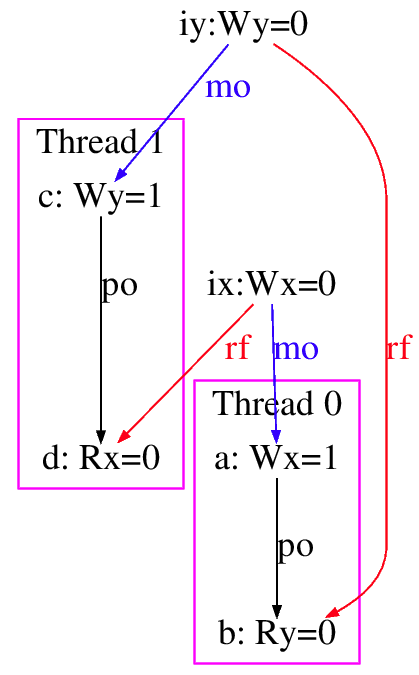
\includegraphics[width=4.5cm]{exec}
	\end{figure}

\end{frame}

\begin{frame}{RC11}

	\vfill
	\begin{itemize}
	\item $\hb ; \eco ^?$ is irreflexive. \hfill (coherence)
	\item $\rmw \cap (\rb ; \mo) = \emptyset$. \hfill (atomicity)
	\item $\psc$ is acyclic. \hfill (sequential-consistency)
	\item $\po \cup \rf$ is acyclic. \hfill (no-thin-air)
	\end{itemize}
	\vfill

\end{frame}

\begin{frame}{Herd}
	\begin{figure}
	\centering
	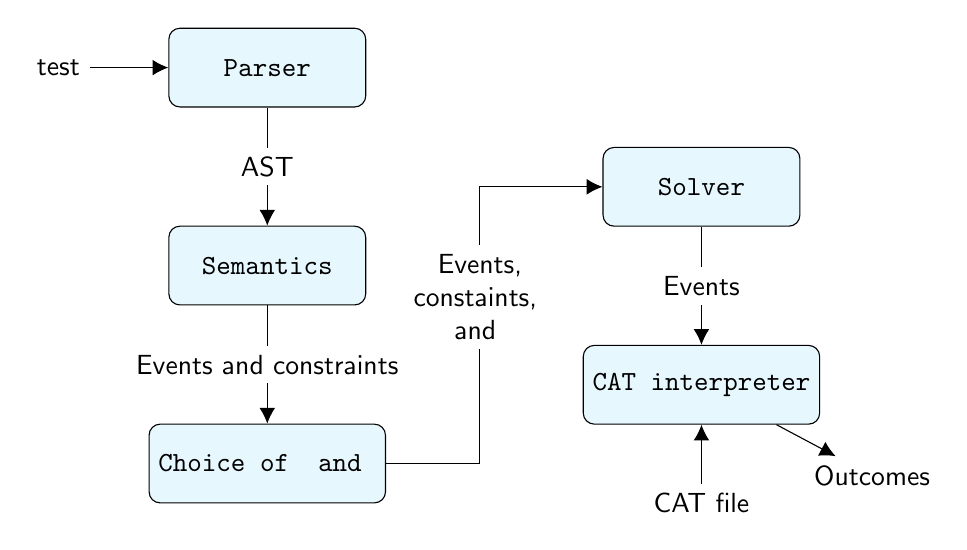
\begin{tikzpicture}[every node/.style={fill=white, font=\sffamily}, node distance=1.5cm, align=center]

	\node (start) [invisible] {test};
	\node (parser) [solid, right = 1cm of start] {Parser};
	\node (sem) [below = of parser, solid] {Semantics};
	\node (choice) [below = of sem, solid] {Choice of $\rf$ and $\mo$};
	\node (solver) [below right = 0.5cm and 3 of parser, solid] {Solver};
	\node (interp) [below = of solver, solid] {CAT interpreter};
	\node (end) [invisible, below right = 0.4cm and -0.2cm of interp] {Outcomes};
	\node (model) [invisible, below of = interp] {CAT file};
	
	\draw[->] (start) -- (parser);
	\draw[->] (parser) -- node {AST} (sem);
	\draw[->] (sem) -- node {Events and constraints} (choice);
	\draw[->] (choice) -| ++(2.7,1) |- node[text width=2cm, minimum size = 0.1cm, yshift=-1.4cm] {Events, constaints, $\mo$ and $\rf$} (solver);
	\draw[->] (solver) -- node {Events} (interp);
	\draw[->] (interp) -- (end);
	\draw[->] (model) -- (interp);
	
	\end{tikzpicture}
	\end{figure}

\end{frame}

\begin{frame}

	Generates every combination of $\rf$ and $\po$, this is computationally expensive
	
	Dealing with large sets of executions is a common problem for model checkers
	
	Solution : a stateless algorithm that avoids this

\end{frame}

\begin{frame}{The stateless algorithm}

	\begin{figure}
	\centering
	
	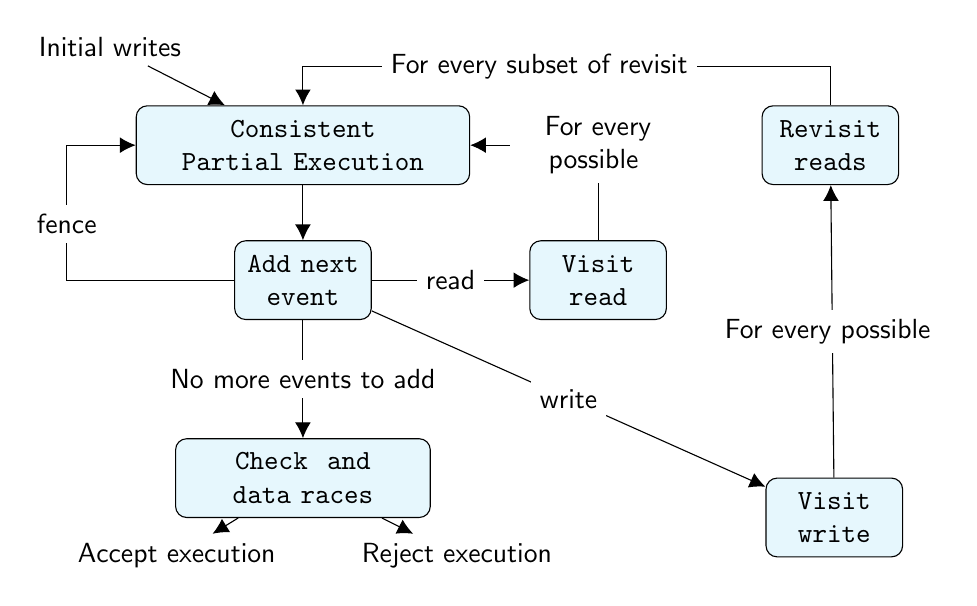
\begin{tikzpicture}[every node/.style={fill=white, font=\sffamily}, node distance=1.5cm, align=center, minimum width = 0]
	
	\node (cpe) [solid, text width = 4cm]{Consistent Partial Execution};
	\node (add) [solid, below = 0.7cm of cpe, text width = 1.5cm, minimum width = 0] {Add next event};
	\node (read) [solid, right = 2cm of add, text width = 1.5cm, minimum width = 0] {Visit read};
	\node (write) [solid, below right = 2cm and 5cm of add, text width = 1.5cm, minimum width = 0] {Visit write};
	\node (revisit) [solid, right = 3.7cm of cpe, text width = 1.5cm, minimum width = 0] {Revisit reads};
	\node (done) [solid, below = of add, text width = 3cm] {Check $\psc$ and data races};
	\node (in) [invisible, above left = 0.5cm and -0.7cm of cpe] {Initial writes};
	\node (accept) [invisible, below left = 0.2cm and -1.4cm of done] {Accept execution};
	\node (reject) [invisible, below right = 0.2cm and -1cm of done] {Reject execution};
	
	
	\draw[->] (cpe) -- (add);
	\draw[->] (add) -- node {read} (read);
	\draw[->] (add) -- node {write} (write);
	\draw[->] (add) -- node {No more events to add} (done);
	\draw[->] (add) -| ++(-3cm,0) |- node[yshift=-1cm] {fence} (cpe);
	\draw[->] (read) |- node[text width = 2cm] {For every possible $\rf$} (cpe);
	\draw[->] (write) -- node {For every possible $\mo$} (revisit);
	\draw[->] (revisit) |- ++(0,1cm) -| node[xshift = 3cm] {For every subset of revisit} (cpe);
	\draw[->] (in) -- (cpe);
	\draw[->] (done) -- (accept);
	\draw[->] (done) -- (reject);
	
	\end{tikzpicture}	
	
	\end{figure}	 

\end{frame}

\end{document}